\documentclass[12pt]{article}
\usepackage{geometry}                % See geometry.pdf to learn the layout options. There are lots.
\geometry{letterpaper}                   % ... or a4paper or a5paper or ... 
%\geometry{landscape}                % Activate for for rotated page geometry
%\usepackage[parfill]{parskip}    % Activate to begin paragraphs with an empty line rather than an indent
\usepackage{float}
\usepackage{graphicx}
\graphicspath{{images/}}
\usepackage{amsmath,amssymb,amsfonts,amsthm} 
\usepackage{epstopdf}
\usepackage{epigraph}
\usepackage{url}
\usepackage{mathtools}

% Computer Concrete
%\usepackage{concmath}
%\usepackage[T1]{fontenc}

% Times variants
%
%\usepackage{mathptmx}
%\usepackage[T1]{fontenc}
%
%\usepackage[T1]{fontenc}
%\usepackage{stix}
%
% Needs to typeset using LuaLaTeX:
%\usepackage{unicode-math}
%\setmainfont{XITS}
%\setmathfont{XITS Math}

% garamond
%\usepackage[cmintegrals,cmbraces]{newtxmath}
%\usepackage{ebgaramond-maths}
%\usepackage[T1]{fontenc}

\DeclareGraphicsRule{.tif}{png}{.png}{`convert #1 `dirname #1`/`basename #1 .tif`.png}

\theoremstyle{plain}
\newtheorem{theorem}{Theorem}
\newtheorem{corollary}[theorem]{Corollary}
\newtheorem{lemma}[theorem]{Lemma}
\newtheorem{proposition}[theorem]{Proposition}
\newtheorem{conjecture}[theorem]{Conjecture}
\newtheorem{question}[theorem]{Question}

\theoremstyle{definition}
\newtheorem{definition}[theorem]{Definition}
\newtheorem{example}[theorem]{Example}
\newtheorem{keywords}{Keywords}
\newtheorem{reference}{Reference}

\theoremstyle{remark}
\newtheorem{remark}[theorem]{Remark}
\newtheorem{note}[theorem]{Note}

%\newcommand{\defeq}{\coloneqq}
\newcommand*{\defeq}{\mathrel{\vcenter{\baselineskip0.5ex \lineskiplimit0pt
                     \hbox{\scriptsize.}\hbox{\scriptsize.}}}
                     =}
\newcommand{\N}{\mathbf N} 
\newcommand{\Q}{\mathbf Q} 
\newcommand{\R}{\mathbf R}

\title{Analysis}
\author{Nhan Trong}
\date{July 3, 2016---\today}                                           % Activate to display a given date or no date

\begin{document}
\sloppy
\maketitle

\epigraph{\textit{In mathematics you don't understand things. You just get used to them.}}{John von Neumann}

\part{Polynomial Approximation}

\begin{theorem}[Taylor's Theorem]
If $f', \ldots, f^{(n+1)}$ are defined on $[a, x]$, then 
$$f(x) = f(a) + f'(a)(x - a) + \cdots + \frac{f^{(n)}(a)}{n!}(x - a)^n + R_n(x)$$
where $R_n(x) = \frac{f^{(n+1)}(t)}{(n+1)!}(x - a)^{n+1}$ for some $t$ in $(a, x)$.
\end{theorem}

\begin{note}
The Mean Value Theorem is a special case of Taylor's Theorem:
$$f(b) = f(a) + f'(c)(b - a)$$
for some $c$ between $a$ and $b$.
\end{note}

\begin{keywords}
Taylor's Theorem, Taylor polynomial, error / remainder term, Cauchy, Lagrange, integral form.
\end{keywords}

\part{Sequences}

\epigraph{\texttt{4 8 15 16 23 42}}{Lost}

\begin{theorem}[Uniform Limit Theorem]
Uniform convergence of functions preserves continuity, i.e. if $f_n$ are continuous and approach $f$ uniformly, then $f$ is continuous.
\end{theorem}

\begin{proposition}
The uniform limit of uniformly continuous functions is uniformly continuous.
\end{proposition}

\begin{question}
What about differentiability, i.e. if $f_n$ are differentiable and approach $f$ uniformly, is $f$ always differentiable, and is $\lim f_n' = f'$? 
\end{question}

\begin{example}
No to the second question: the functions $f_n(x) = \frac{1}{n} \sin(nx)$ converge uniformly to the zero function, which \textit{is} differentiable. But, the limit of the derivatives don't exist. What about just differentiability? 
\end{example}

\centerline{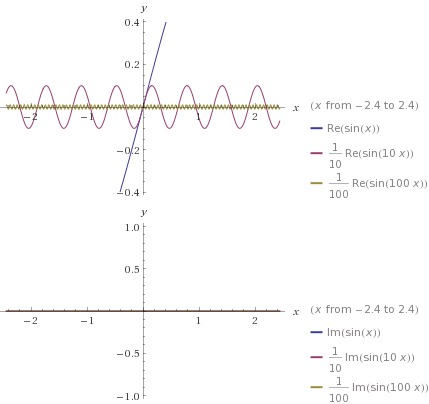
\includegraphics[width=1.0\textwidth]{uniformconvergence1}}

\begin{example}
Still No, e.g. the functions $f_n(x) = \sqrt{x^2 + 1/n}$ converge uniformly to $f = |x|$, which is not differentiable at zero.
\end{example}

\centerline{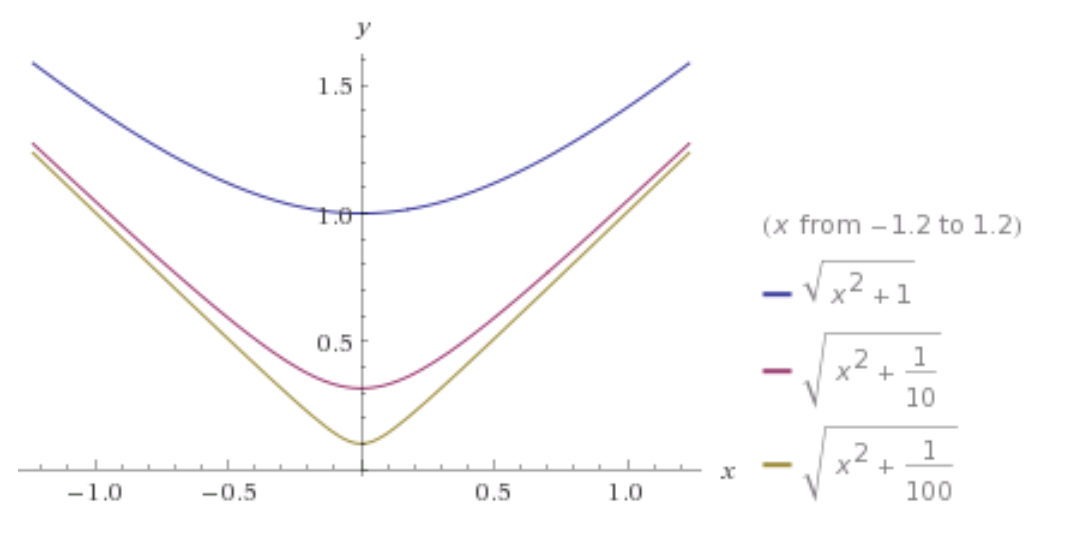
\includegraphics[width=1.0\textwidth]{uniformconvergence2}}

\begin{example}[Weierstrass function]
The Weierstrass function $$f(x) = \sum^\infty_{k=0} a^k \cos(b^k \pi x),$$ for appropriate values $a$ and $b$, is the uniform limit of $$f_n = \sum^n_{k=0} a^k \cos(b^k \pi x),$$ but is nowhere differentiable.
\end{example}

\centerline{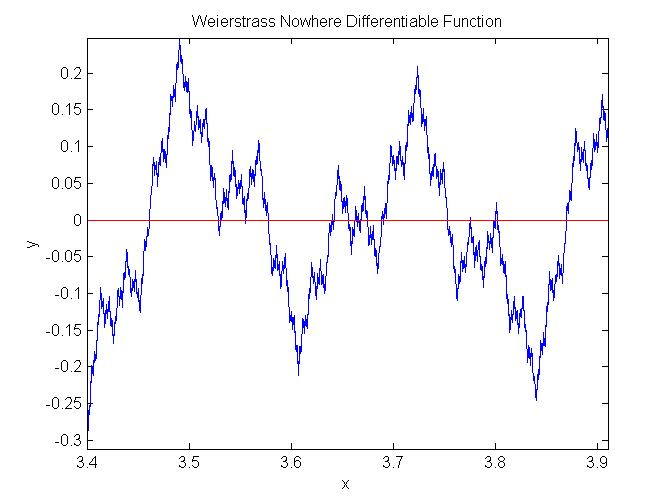
\includegraphics[width=1.0\textwidth]{nodiff1}}

\begin{question}
Is the Koch snowflake nowhere differentiable?
\end{question}

Yes. Proof?

\centerline{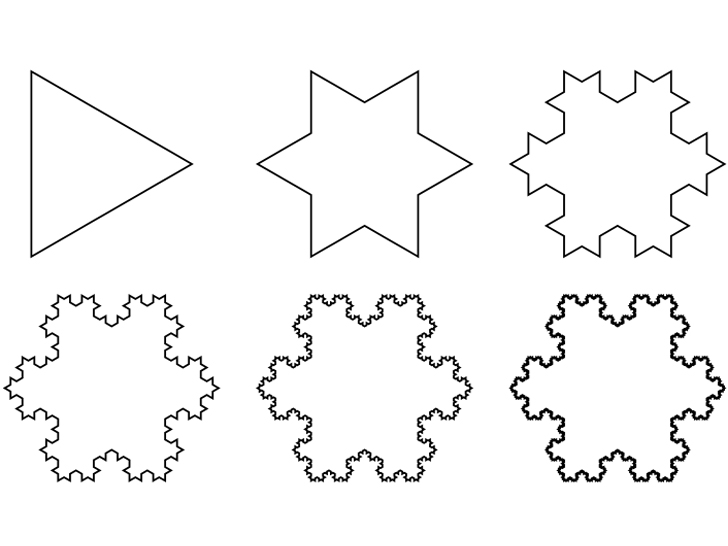
\includegraphics[width=1.0\textwidth]{biomimicry-koch-snowflake}}

\begin{definition}
Let $\{a_n\}$ be a sequence, and $0 \leq a < b \leq 1$. Let $N(n; a, b)$ be the number of integers $j \leq n$ s.t. $a_j \in [a, b].$ A sequence $\{a_n\}$ of numbers in $[0, 1]$ is called uniformly distributed in $[0, 1]$ if $$\lim_{n \to \infty} \frac{N(n; a, b)}{n} = b - a$$ for all $a, b,$ s.t. $0 \leq a < b \leq 1.$
\end{definition}

\begin{proposition}
If $s$ is a step function on $[0, 1]$, and $\{a_n\}$ is uniformly distributed in $[0, 1]$, then $$\int_0^1 s = \lim_{n\to\infty} \frac{s(a_1) + \cdots + s(a_n)}{n}.$$
\end{proposition}

\begin{proof}
Let $\Delta_1, \ldots, \Delta_m$ be a partition of $[0, 1]$ corresponding to the steps in $s.$ Then (with a slight abuse of notation) we have 
\begin{align*}
\int_0^1 s &= \sum_{i=1}^m s(\Delta_i) \Delta_i \\
&= \sum_{i=1}^m s(\Delta_i) \lim_{n \to \infty} \frac{1}{n} N(n; \Delta_i) \\
&= \lim_{n \to \infty} \frac{1}{n} \sum_{i=1}^m s(\Delta_i) N(n; \Delta_i) \\
&= \lim_{n \to \infty} \frac{1}{n} \sum_{i=1}^n s(a_i).\qedhere
\end{align*}
\end{proof}

\begin{proposition}
If $f$ is integrable on $[0, 1]$, and $\{a_n\}$ is uniformly distributed in $[0, 1]$, then $$\int_0^1 f = \lim_{n\to\infty} \frac{f(a_1) + \cdots + f(a_n)}{n}.$$
\end{proposition}

\begin{proof}[Sketch]
Since $f$ is integrable, there is a step function $s$ such that $\int_0^1 f$ is close to $\int_0^1 s$, which is close to $\frac{s(a_1) + \cdots + s(a_n)}{n}$, which is close to $\frac{f(a_1) + \cdots + f(a_n)}{n}$.
\end{proof}

\section{Bolzano-Weierstrass Theorem}

\begin{theorem}[Bolzano-Weierstrass Theorem]
An infinite sequence contained in a closed interval $I$ has a limit point in $I.$
\end{theorem}

\begin{figure}[H]
\centering
\includegraphics[width=.5\textwidth]{Bolzano–Weierstrass_theorem_-_step_7}
\end{figure}

Proof uses the Nested Interval Theorem:

\begin{theorem}[Nested Interval Theorem]
The intersection of closed nested intervals is nonempty. If the interval lengths tend to zero, then the intersection is a point. Otherwise it's a closed interval.
\end{theorem}

\begin{figure}[H]
\centering
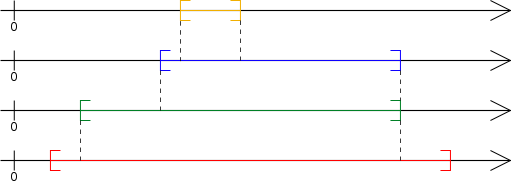
\includegraphics[width=1.0\textwidth]{511px-Illustration_nested_intervals}
\end{figure}

\begin{definition}
A function $f$ defined on an interval $I$ is called limitful if $\lim\limits_{y\to a} f(y)$ exists for all $a \in I$.
\end{definition}

\begin{proposition}
Let $f$ be a limitful function on $[0, 1]$. Then for any $\epsilon > 0$ there are only finitely many points $a \in [0, 1]$ with $$|\lim\limits_{y\to a} f(y) - f(a)| > \epsilon.$$
\end{proposition}

\begin{proof}[Sketch 1]
Suppose that there are infinitely many such points $a.$ Then by the Bolzano-Weierstrass Theorem, these points have a limit $x \in [0, 1].$ Let $$L \defeq \lim\limits_{y \to x} f(y) = \lim\limits_{a\to x} f(a).$$

The condition $$|\lim\limits_{y\to a} f(y) - f(a)| > \epsilon$$ means that for $y$ close to $a$, $f(y)$ is far from $f(a).$ Similarly $\lim\limits_{a \to x} f(a) = L$ means that for $a$ close to $x,$ $f(a)$ is close to $L.$ Together this means that for $y$ close to $x$ and $y$ close to $a$ for some $a$, we have that $f(y)$ is far from $L$, but this contradicts the fact that $L = \lim\limits_{y \to x} f(y),$ i.e. for all $y$ close to $x$, $f(y)$ is close to $L.$
\end{proof}

\begin{proof}[Sketch 2]
Another way to see this is to let $a_n$ be the convergent subsequence given by Bolzano-Weierstrass, and choose $y_n$ close to $a_n$ so that $|f(y_n) - f(a_n)|$ is big. Since $|f(a_n) - L|$ is small, the triangle inequality 
$$|f(y_n) - L| \geq |f(y_n) - f(a_n)| - |f(a_n) - L|$$ 
says $|f(y_n) - L|$ is big, thus contradiction.
\end{proof}

\begin{theorem}
A limitful function on $[0, 1]$ has at most countably many discontinuities.
\end{theorem}

\begin{proof}
By the previous Proposition, for each $\epsilon_q > 0$ there are at most finitely many points $a$ s.t. $$|\lim\limits_{y\to a} f(y) - f(a)| > \epsilon_q.$$ Taking a sequence $\epsilon_q \in \Q$ converging to zero, we have countably many such points $a$.
\end{proof}

\begin{corollary}
If $f$ has only removable discontinuities, then $f$ is continuous except at countably many points. In particular, $f$ cannot be discontinuous everywhere.
\end{corollary}

\section{Keywords}

Uniform Limit Theorem, point-wise, uniform convergence, metric space, Cauchy criterion, Koch snowflake, Weierstrass function, uniformly distributed / equidistributed sequence, Bolzano-Weierstrass / Sequential Compactness Theorem, limitful function, removable discontinuity.

\part{Infinite Series}

\epigraph{\textit{Infinite growth of material consumption in a finite world is an impossibility.}}{E. F. Schumacher}

\begin{thebibliography}{99}

\bibitem{spivak} Spivak's Calculus.

\end{thebibliography}

\end{document}
